%%%%%%%%%%%%%%%%%%%%%%%%%%%%%%%%%%%%%%%%%
% Short Sectioned Assignment LaTeX Template Version 1.0 (5/5/12)
% This template has been downloaded from: http://www.LaTeXTemplates.com
% Original author:  Frits Wenneker (http://www.howtotex.com)
% License: CC BY-NC-SA 3.0 (http://creativecommons.org/licenses/by-nc-sa/3.0/)
%%%%%%%%%%%%%%%%%%%%%%%%%%%%%%%%%%%%%%%%%

%----------------------------------------------------------------------------------------
%   PACKAGES AND OTHER DOCUMENT CONFIGURATIONS
%----------------------------------------------------------------------------------------

\documentclass[10pt,a4paper,spanish]{article}

% ---- Entrada y salida de texto -----

\usepackage[spanish]{babel} 
\usepackage[T1]{fontenc} % Use 8-bit encoding that has 256 glyphs
\usepackage[utf8]{inputenc}
\usepackage{minted}
% \usepackage{fourier} % Use the Adobe Utopia font for the document - comment this line to return to the LaTeX default
\usepackage[usenames, dvipsnames]{color}
\usepackage{xcolor}
\usepackage{colortbl}
\usepackage[bookmarks=true,colorlinks=true,linkcolor=red,citecolor=blue]{hyperref}
\usepackage{cite}
\usepackage[official]{eurosym}
\usepackage{tikz}
\usepackage{pgfplots}
\pgfplotsset{compat=1.5}
% \usepackage{pgf-pie}
\usepackage{subfigure}

% ---- Otros paquetes ----
\usepackage{enumerate}
\usepackage{amsmath,amsfonts,amsthm,amssymb} % Math packages
\usepackage{graphics,graphicx} %para incluir imágenes y notas en las imágenes
% Para hacer tablas comlejas
%\usepackage{multirow}
%\usepackage{threeparttable}

\usepackage[a4paper, margin=1.3in]{geometry}


\usepackage{sectsty} % Allows customizing section commands
\allsectionsfont{\centering \normalfont\bfseries\scshape} % Make all sections centered, the default font and small caps

\usepackage{fancyhdr} % Custom headers and footers
\pagestyle{fancyplain} % Makes all pages in the document conform to the custom headers and footers
\fancyhead{} % No page header - if you want one, create it in the same way as the footers below
\fancyfoot[L]{} % Empty left footer
\fancyfoot[C]{} % Empty center footer
\fancyfoot[R]{\thepage} % Page numbering for right footer
\renewcommand{\headrulewidth}{0pt} % Remove header underlines
\renewcommand{\footrulewidth}{0pt} % Remove footer underlines
\setlength{\headheight}{13.6pt} % Customize the height of the header

\numberwithin{equation}{section} % Number equations within sections (i.e. 1.1, 1.2, 2.1, 2.2 instead of 1, 2, 3, 4)
\numberwithin{figure}{section} % Number figures within sections (i.e. 1.1, 1.2, 2.1, 2.2 instead of 1, 2, 3, 4)
\numberwithin{table}{section} % Number tables within sections (i.e. 1.1, 1.2, 2.1, 2.2 instead of 1, 2, 3, 4)

\setlength\parindent{0pt} % Removes all indentation from paragraphs - comment this line for an assignment with lots of text
\setlength{\parskip}{1ex plus 0.5ex minus 0.2ex}

\newcommand{\horrule}[1]{\rule{\linewidth}{#1}} % Create horizontal rule command with 1 argument of height

%----------------------------------------------------------------------------------------
%   TÍTULO Y DATOS DEL ALUMNO
%----------------------------------------------------------------------------------------

\title{
\normalfont \normalsize 
\textsc{{\bf Ingeniería de Servidores (2015-2016)} \\ Grado en Ingeniería Informática \\ Universidad de Granada} \\ [25pt] % Your university, school and/or department name(s)
\horrule{0.5pt} \\[0.4cm] % Thin top horizontal rule
\huge Memoria Práctica 3 \\ % The assignment title
\horrule{2pt} \\[0.5cm] % Thick bottom horizontal rule
}

\author{Marta Gómez Macías} % Nombre y apellidos

\date{\normalsize\today} % Incluye la fecha actual

\newmintedfile[mybash]{bash}{
    linenos,
    numbersep=5pt,
    gobble=0,
    frame=lines,
    framesep=2mm,
    tabsize=3,
}

\newmintedfile[myyml]{yaml}{
    linenos,
    numbersep=5pt,
    gobble=0,
    frame=lines,
    framesep=2mm,
    tabsize=3,
}

\newmintedfile[mypython]{python}{
    linenos,
    numbersep=5pt,
    gobble=0,
    frame=lines,
    framesep=2mm,
    tabsize=3,
}

%----------------------------------------------------------------------------------------
% DOCUMENTO
%----------------------------------------------------------------------------------------

\begin{document}
%Cambiar Cuadros por Tablas y lista de...
\renewcommand{\listtablename}{Índice de tablas}
% \renewcommand{\tablename}{Tabla} 

\maketitle % Muestra el Título
\pagenumbering{gobble} 

\newpage %inserta un salto de página
\pagenumbering{arabic} 

\tableofcontents % para generar el índice de contenidos

\listoffigures

% \listoftables

\newpage

\section{a) ¿Qué archivo le permite ver qué programas se han instalado con el gestor de paquetes? b) ¿Qué significan las terminaciones 1.gz o 2.gz de los archivos en ese directorio?}

\begin{enumerate}[a)]
    \item En el caso de CentOS, el archivo de log de yum, que se encuentra en \textit{/var/log/yum.log}. En la \hyperref[yumlog]{Figura \ref*{yumlog}} se ve, por ejemplo, que el día 30 de Octubre instalé el paquete \texttt{screen}.

    En el caso de Ubuntu, el archivo correspondiente sería \textit{/var/log/apt/history.log}. En la \hyperref[aptlog]{Figura \ref*{aptlog}}, se ve como, por ejemplo, el día 8 de Noviembre eliminé el paquete \texttt{python-pip}.

    \begin{figure}[!h]
    \centering
    \mbox {
    \subfigure[Archivo bitácora de Yum, en el que vemos un histórico de todos los paquetes instalados, actualizados y eliminados]{
    \label{yumlog}
    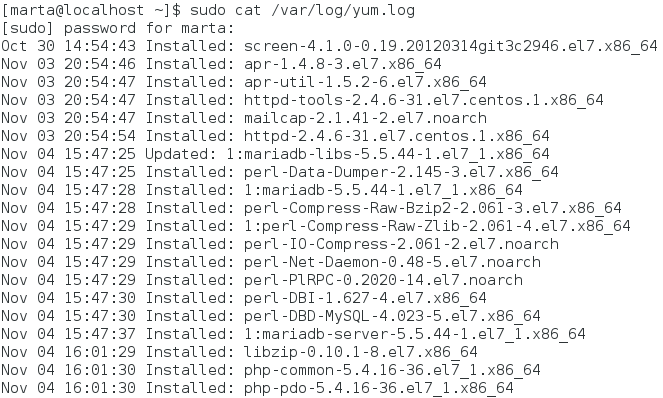
\includegraphics[width=0.5\textwidth]{1}
    }
    \qquad
    \subfigure[Archivo bitácora de Apt, con el historial de todos los paquetes descargados, instalados, actualizados y eliminados] {
    \label{aptlog}
    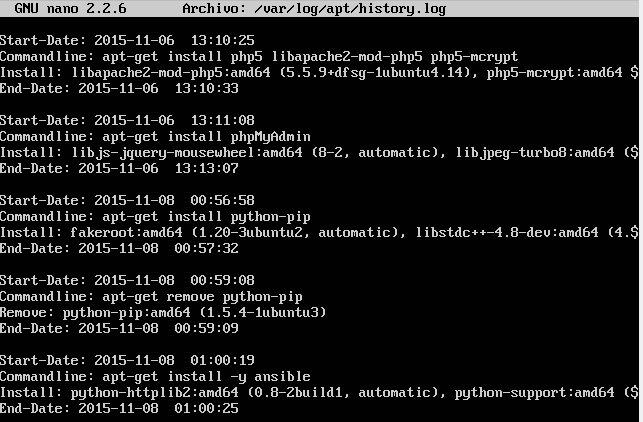
\includegraphics[width=0.5\textwidth]{2}
    }
    }
    \caption{Consultando el historial de operaciones hechas con los gestores de paquetes}
    \label{gestordepaquetes}
    \end{figure}

    \item Tal y como se indica en \cite{logrotation}, la existencia de dichos archivos se debe a que nuestro sistema está programado para llamar al comando \texttt{logrotate} cada $x$ tiempo con \texttt{cron}. Estos archivos son antiguos logs que se han dejado ahí por si el administrador quiere consultarlos. Cada determinado tiempo, el archivo log se renombra y se crea uno nuevo, éste antiguo se comprime usando \texttt{gzip}. Así conseguimos que el archivo de logs no tenga un tamaño demasiado grande y podemos tener nuestros logs clasificados según el tiempo que queramos (por ejemplo, cada día se crea un nuevo archivo de log, y si queremos consultar los del día pasado consultaríamos el que tuviese la terminación \texttt{1.gz}).
\end{enumerate}

\section{¿Qué archivo ha de modificar para programar una tarea? Escriba la lína necesaria para ejecutar una vez al día una copia del directorio \textit{$\sim$/codigo} a \textit{$\sim$/seguridad/\$fecha} donde \textit{\$fecha} es la fecha actual (puede usar el comando \texttt{date}).}
Tal y como se indica en \cite{crontab}, los archivos \textit{crontab} de cada usuario se encuentran en \textit{/var/spool/cron/crontabs/}. Sin embargo, no se recomienda editar directamente estos archivos, sino hacerlo a través del comando \texttt{crontab}. Además, como también se indica en \cite{cron}, no es necesario reiniciar \texttt{cron} cuando modificamos el \texttt{crontab}.

Para hacer la tarea, hemos ejecutado con la opción \texttt{-e} para editar el archivo \texttt{crontab} del usuario actual
\begin{minted}[frame=single, label={Llamando a crontab}]{console}
$ crontab -e
\end{minted}
Tras esto, escribimos en el editor \texttt{nano} la siguiente línea:
\begin{minted}{bash}
14 22 * * * cp -R $HOME/codigo/ $HOME/seguridad/"$(date)"
\end{minted}

En la \hyperref[cronprueba]{Figura \ref*{cronprueba}} se ven dos capturas de pantalla del contenido del directorio \textit{home} del servidor, antes y después de que cron actúe. Como se ve, tras actuar cron se crea una carpeta con la fecha actual dentro del directorio \textit{servidor} y con el mismo contenido que código.

\begin{figure}[!h]
\centering
\mbox {
\subfigure[Comando \texttt{ls -l} ejecutado antes de la hora de acción de crontab]{
\label{lsl}
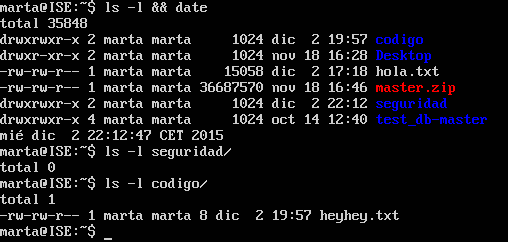
\includegraphics[width=0.5\textwidth]{44}
}
\qquad
\subfigure[Comando \texttt{ls -l} ejecutado después de la hora de acción de crontab] {
\label{lsl1}
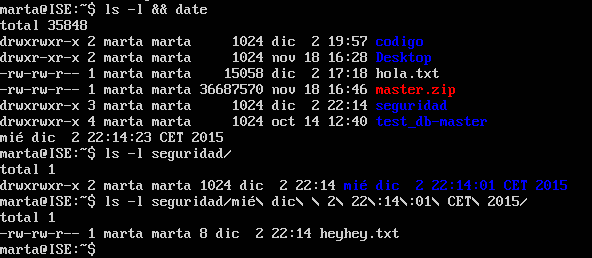
\includegraphics[width=0.5\textwidth]{45}
}
}
\caption{Consultando el historial de operaciones hechas con los gestores de paquetes}
\label{cronprueba}
\end{figure}

\section{Pruebe a ejecutar el comando \texttt{dmesg}, conectar un dispositivo USB y vuelva a ejecutar el comando. Copie y pegue la salida del comando. (Considere usar \texttt{dmesg | tail}). Comente qué observa en la información mostrada.}
Nada más iniciar el sistema y ejecutar \texttt{dmesg | tail}, he obtenido la información de la \hyperref[dmesg1]{Figura \ref*{dmesg1}}. En ella nos muestra información sobre cómo configura la red WiFi al arrancar.

\begin{figure}[!h]
    \centering
    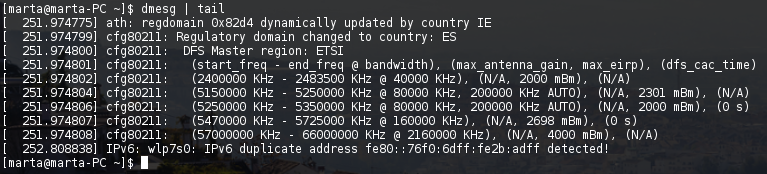
\includegraphics[width=1\textwidth]{7}
    \caption{Información mostrada por \texttt{dmesg | tail} nada más iniciar el sistema}
    \label{dmesg1}
\end{figure}

Tras conectar una memoria USB al ordenador y volver a ejecutar el comando \texttt{dmesg | tail}, vemos la información mostrada en la \hyperref[dmesg2]{Figura \ref*{dmesg2}}. En la foto vemos cómo ha reconocido el pen drive y realiza las operaciones necesarias para montarlo en memoria, también nos lanza un aviso de que \texttt{umount} no funcionó correctamente sobre el sistema de archivos FAT. Sin embargo, aún no habíamos desmontado la memoria USB. Tras desconectar la memoria USB y volver a ejecutar \texttt{dmesg | tail} obtenemos, además de la información de la \hyperref[dmesg2]{Figura \ref*{dmesg2}}, la información de la \hyperref[dmesg3]{Figura \ref*{dmesg3}}.

\begin{figure}[!h]
    \centering
    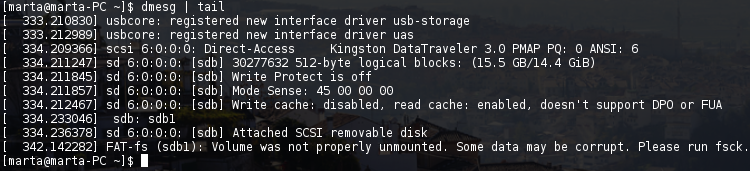
\includegraphics[width=1\textwidth]{8}
    \caption{Información mostrada por \texttt{dmesg | tail} al conectar una memoria USB al ordenador}
    \label{dmesg2}
\end{figure}

\begin{figure}[!h]
    \centering
    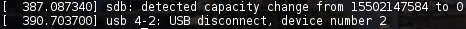
\includegraphics[width=0.7\textwidth]{9}
    \caption{Información adicional añadida cuando ejecutamos \texttt{dmesg | tail} tras desconectar la memoria USB}
    \label{dmesg3}
\end{figure}

\section{Ejecute el monitor \texttt{perfmon} de ``Systen Performance'' y muestre el resultado. Incluya capturas de pantalla comentando la información que aparece.}
El monitor nos genera un amplio informe sobre el rendimiento del sistema, el cual está dividido en distintas secciones. La primera parte se ve en la \hyperref[perfmon1]{Figura \ref*{perfmon1}}, donde nos muestra el equipo, la fecha y la duración del análisis; un resumen de los datos obtenidos y un análisis del rendimiento del sistema. En nuestro caso, como sólo estábamos ejecutando el monitor nos da como resultado poca actividad en el sistema.

\begin{figure}[!h]
    \centering
    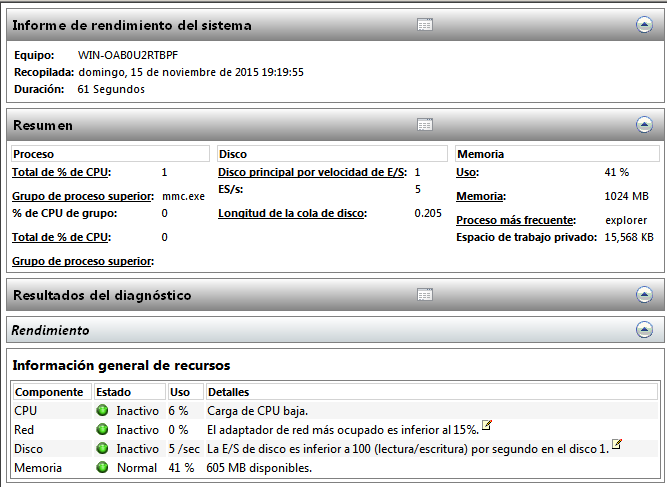
\includegraphics[width=0.75\textwidth]{10}
    \caption{Resumen inicial de los datos obtenidos por el monitor}
    \label{perfmon1}
\end{figure}

% En la segunda parte, nos muestra información detallada con el siguiente orden y jerarquía:
% \begin{enumerate}[$\bullet$]
%     \item CPU
%     \begin{enumerate}[$\circ$]
%         \item Proceso
%         \item Servicio
%         \item Servicios
%         \item Sistema
%     \end{enumerate}
%     \item Red
%     \begin{enumerate}[$\circ$]
%         \item Interfaz
%         \item IP
%         \item TCP
%         \item UDP
%     \end{enumerate}
%     \item Disco
%     \begin{enumerate}[$\circ$]
%         \item Archivos activos
%         \item División de disco
%         \item Disco físico
%     \end{enumerate}
%     \item Memoria
%     \begin{enumerate}[$\circ$]
%         \item Proceso
%         \item Contadores
%     \end{enumerate}
%     \item Estadísticas de informe
%     \begin{enumerate}[$\circ$]
%         \item Información del equipo
%         \item Información recopilada
%         \item Archivos
%         \item Eventos procesados
%     \end{enumerate}
% \end{enumerate}

\section{Cree un recopilador de datos definido por el usuario  en \texttt{perfmon} (modo avanzado) que incluya tanto el contador de rendimiento como los datos de seguimiento: todos los referentes al procesador, al proceso y al servicio web. Intervalo de muestra de 15 segundos. Almacene el resultado en el directorio \textit{Escritorio\textbackslash logs}. Incluya capturas de pantalla de cada paso.}

\begin{enumerate}[1.]
    \item En primer lugar, para entrar al asistente, hacemos click derecho en el submenú \textit{\textbf{Definidos por el usuario}} del menú \textbf{\textit{Conjuntos de recopiladores de datos}}. En dicho submenú seguimos la ruta \textbf{Nuevo $>$ Conjunto de recopiladores de datos} (\hyperref[asistente]{Figura \ref*{asistente}}). Alternativamente podemos hacer click en el botón de \textbf{Nuevo conjunto de recopiladores de datos}.

    \begin{figure}[!h]
        \centering
        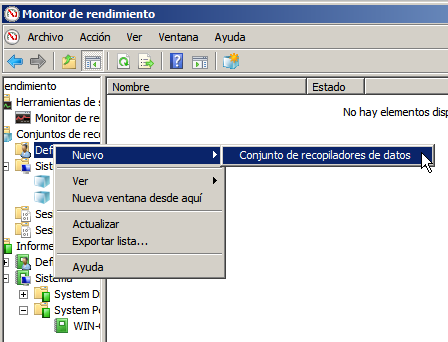
\includegraphics[width=0.7\textwidth]{11}
        \caption{Ruta a seguir para llegar al asistente de creación de nuevo conjunto de recopiladores de datos}
        \label{asistente}
    \end{figure}

    \item Tras esto, saldrá la ventana que vemos en la \hyperref[ventana]{Figura \ref*{ventana}}. En ella, establecemos un nombre para nuestro Conjunto de recopiladores de datos y seleccionamos la opción manual.

    \begin{figure}[!h]
        \centering
        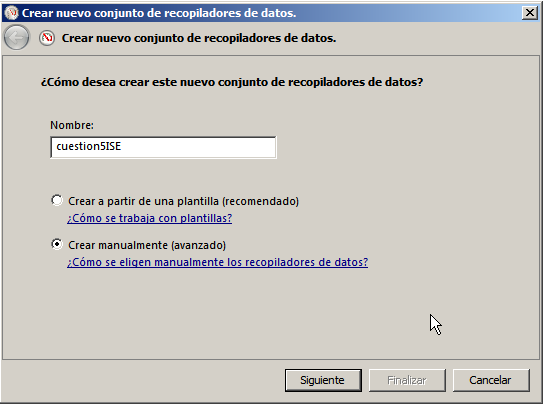
\includegraphics[width=0.7\textwidth]{12}
        \caption{Primer paso para crear un conjunto de recopiladores de datos}
        \label{ventana}
    \end{figure}

    \item Después, veremos la ventana de la \hyperref[window]{Figura \ref*{window}}, en la cual seleccionaremos los datos que queremos recopilar. En nuestro caso seleccionamos los indicados en el guión de prácticas.

    \begin{figure}[!h]
        \centering
        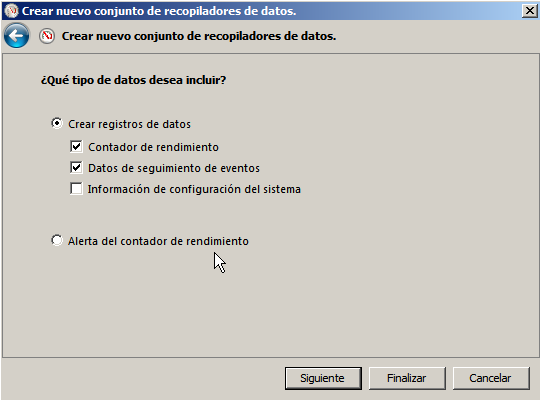
\includegraphics[width=0.7\textwidth]{13}
        \caption{Selección de los datos que queremos recopilar}
        \label{window}
    \end{figure}

    \item Tras darle a siguiente, nos saldrá una ventana en la que tendremos que hacer click en el botón de \textbf{Agregar}. Tras esto nos saldrá una ventana como la que se ve en la \hyperref[addvars]{Figura \ref*{addvars}}. En nuestro caso, mediremos variables sobre el procesador, los procesos y el servicio web. Finalmente, cuando aceptemos volveremos a la ventana anterior, pero esta vez nos mostrará los contadores de rendimiento escogidos (\hyperref[setcountertime]{Figura \ref*{setcountertime}}). El intervalo de muestra por defecto es el deseado en la práctica, por lo que no lo modificamos.
    \begin{figure}[!h]
    \centering
    \mbox {
    \subfigure[Agregando variables a analizar a nuestro recopilador de datos]{
    \label{addvars}
    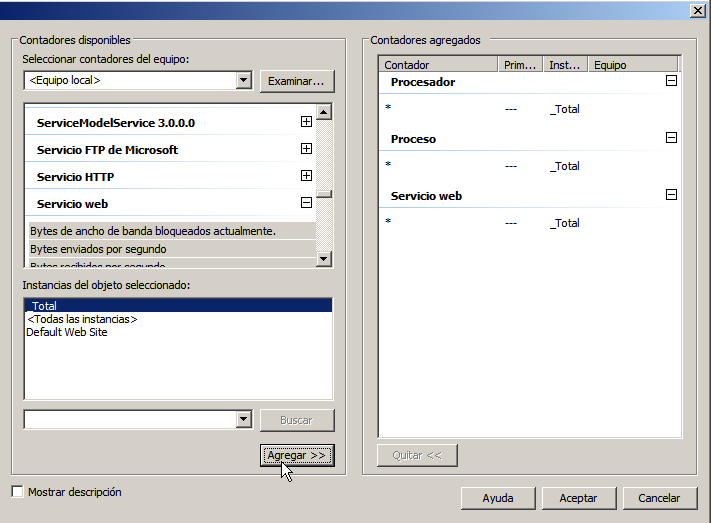
\includegraphics[width=0.5\textwidth]{14}
    }
    \qquad
    \subfigure[Estableciendo los contadores de rendimiento y el intervalo de muestra] {
    \label{setcountertime}
    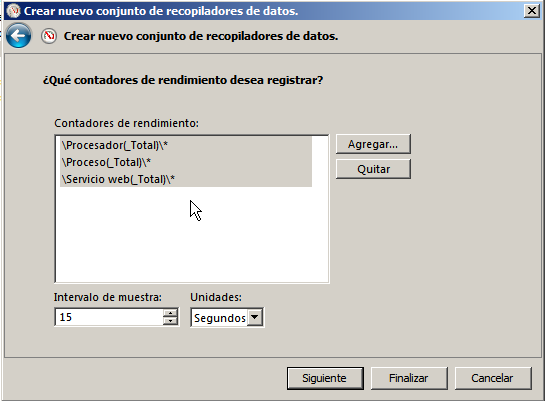
\includegraphics[width=0.5\textwidth]{15}
    }
    }
    \caption{Ultimando los detalles del conjunto de recopiladores de datos creado.}
    \label{ultimopaso}
    \end{figure}

    \item En la siguiente ventana nos preguntará sobre \textit{Proveedores de seguimiento de eventos}. Como no se pide habilitar ninguno, dejamos todo por defecto y le damos a \textbf{Siguiente}.

    \item Después, debemos especificar dónde guardar los \textit{logs}. En nuestro caso debe de ser en una carpeta llamada logs y ubicada en el escritorio (\hyperref[saveplace]{Figura \ref*{saveplace}}).

    \begin{figure}
        \centering
        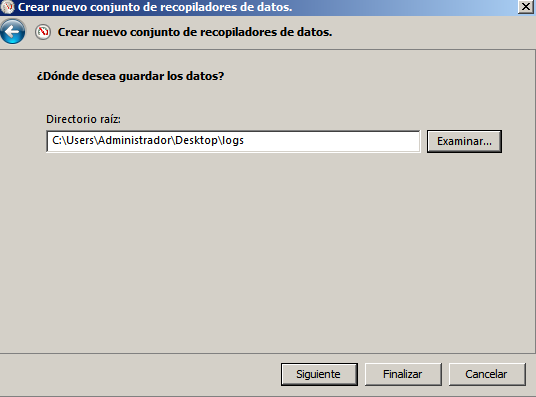
\includegraphics[width=0.7\textwidth]{46}
        \caption{Estableciendo dónde almacenar los logs}
        \label{saveplace}
    \end{figure}

    \item Por último, en la siguiente ventana lo dejamos todo por defecto y hacemos click en \textbf{Finalizar}.

    \item Una vez finalizado, hacemos click derecho sobre nuestro recopilador de datos y entramos al menú \textbf{Propiedades}. Ahí seleccionamos la pestaña \textbf{Detener condición} y establecemos la duración total a 1 minuto (\hyperref[fullmuestra]{Figura \ref*{fullmuestra}}). Si no hacemos esto el recopilador de datos estará eternamente recopilando datos.

    \begin{figure}
        \centering
        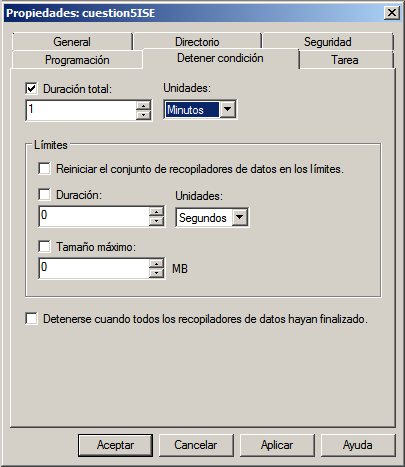
\includegraphics[width=0.5\textwidth]{48}
        \caption{Estableciendo la duración total de la muestra}
        \label{fullmuestra}
    \end{figure}    
\end{enumerate}

Para ejecutar el recopilador de datos que hemos hecho, lo seleccionamos y hacemos click en el botón de \textbf{Iniciar}.

\begin{figure}
    \centering
    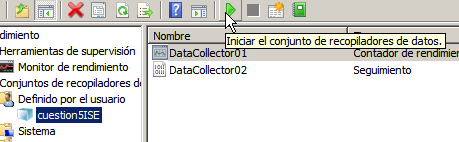
\includegraphics[width=0.7\textwidth]{47}
    \caption{Iniciando el recopilador de datos.}
    \label{startrecopi}
\end{figure} 

Tras finalizar la toma de datos, en la carpeta de \textit{logs} ubicada en el escritorio podremos encontrar los datos obtenidos. El archivo final de datos obtenido se ve en la \hyperref[dataanalisis]{Figura \ref*{dataanalisis}}. Poniendo el ratón sobre cada una de las líneas de la gráfica podemos ver con qué medida se corresponde. Así por ejemplo, el pico azul que se ve en la imagen se corresponde con las operaciones de E/S, en este caso ha habido un aumento del número de lecturas de ficheros sobre el disco duro sobre las 8:52 de la tarde. En cambio, el color fucsia se corresponde con el número de escrituras, que se ha reducido sobre esa misma hora.

\begin{figure}
    \centering
    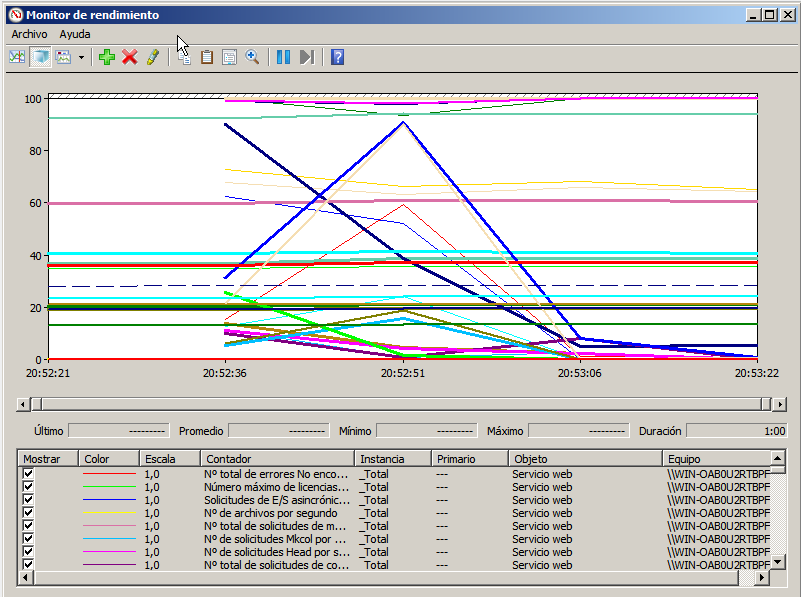
\includegraphics[width=0.7\textwidth]{49}
    \caption{Analizando los datos recopilados}
    \label{dataanalisis}
\end{figure} 

\section{Instale alguno de los monitores comentados arriba en su máquina y pruebe a ejecutarlos (tenga en cuenta que si lo hace en la máquina virtual los resultados pueden no ser realistas). Alternativamente, busque otros monitores para hardware comerciales o de código abierto para Windows y Linux}
\subsection{Instalando y probando monitores hardware}
\subsubsection{\texttt{hddtemp}}
En \cite{hddtemp} se explica un uso básico de éste monitor. Su sintaxis requiere de, al menos, la ruta de un dispositivo de disco duro para monitorizar. Nosotros usaremos \texttt{/dev/sda1}. El resultado obtenido es el de la \hyperref[hddtemp1]{Figura \ref*{hddtemp1}}, $35^{\circ}$ que es una temperatura bastante buena.

\begin{figure}[!h]
    \centering
    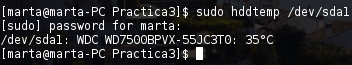
\includegraphics[width=0.5\textwidth]{16}
    \caption{Resultado tras ejecutar \texttt{hddtemp} sobre el disco duro del ordenador}
    \label{hddtemp1}
\end{figure}

\subsubsection{\texttt{xsensors}}
Con \texttt{xsensors} podemos ver la temperatura de los distintos procesadores que tenemos en el ordenador cada segundo. Podemos cambiar el tiempo de refresco con la opción \texttt{-t}.

Al ejecutar \texttt{xsensors} obtenemos la ventana de la 

\begin{figure}[!h]
\centering
\mbox {
\subfigure[Pestaña en la que vemos la temperatura de la placa base en la zona de la CPU]{
\label{xsensors1}
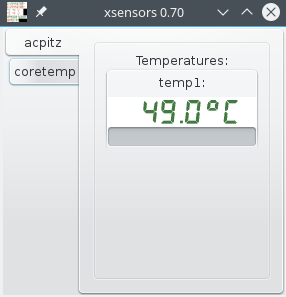
\includegraphics[width=0.25\textwidth]{18}
}
\qquad
\subfigure[Pestaña en la que medimos la temperatura de los procesadores] {
\label{aptlog}
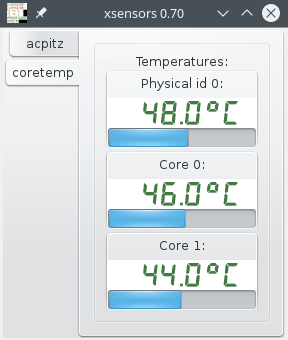
\includegraphics[width=0.25\textwidth]{17}
}
}
\caption{Ejecutando \texttt{xsensors}}
\label{xsensors}
\end{figure}

Al ejecutar el script \texttt{sensors-detect}, según \cite{archsensors}, podemos detectar los distintos sensores que tienen incorporados nuestro hardware para realizar mediciones. En mi caso, como se ve en la \hyperref[sensorsdetect]{Figura \ref*{sensorsdetect}}, sólo detecta los ya mostrados.

\begin{figure}[!h]
    \centering
    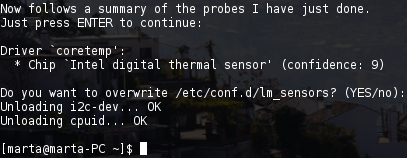
\includegraphics[width=0.5\textwidth]{19}
    \caption{Resumen final de los sensores detectados}
    \label{sensorsdetect}
\end{figure}

\subsection{Otros monitores hardware}
\subsubsection{Smartmontools}
En \cite{linuxhw}, se citan algunos monitores hardware y comandos para saber el hardware del que disponemos en Linux. Uno de los monitores de los que se habla es \textbf{Smartmontools}, que sirve para probar el correcto funcionamiento de nuestro disco duro, para ello ejecutan pruebas y leen datos que el propio disco guarda para su monitorización. Tiene una interfaz gráfica llamada \textit{SmartControl}. Éste monitor también está disponible para Windows.

\subsubsection{Hmonitor}
Éste monitor sólo se encuentra disponible para Windows, en su \href{http://hmonitor.com/}{página web} encontramos una breve explicación de su funcionalidad:
\begin{enumerate}[$\bigstar$]
    \item Monitor de temperatura, que usa los sensores integrados en el hardware para saber su temperatura.
    \item Alerta (o ejecución de una acción definida por el usuario) cuando algún componente alcanza una temperatura más alta de lo normal
    \item Nos puede mostrar gráficos sobre la actividad del procesador y su temperatura con la utilidad \textit{W2K PerfMon}.
\end{enumerate}

\section{Visite la web del proyecto \textit{Munin} y acceda a la demo que proporcionan donde se muestra cómo monitorizan un servidor. Monitorice varios parámetros y haga capturas de pantalla de lo que está mostrando comentando qué observa.}
En la demo, sólo podemos consultar valores ya monitorizados, pero no podemos escribir datos ni hacer nuevas monitorizaciones. Los datos que podemos consultar están en el menú de la izquierda puestos por categorías: podemos consultar problemas que haya encontrado Munin, los datos organizados según el servidor en el que se esté midiendo, los datos organizados según grupos (red, disco, logins, etc.). Éstos datos pueden consultarse según día, mes, año, etc. Ésta interfaz que describo se ve en la \hyperref[iniciomunin]{Figura \ref*{iniciomunin}}. En este caso, Munin ha encontrado una advertencia que darnos, estamos midiendo datos en tres servidores distintos (munin-monitoring.org, vm y vpn) y tenemos varias categorias.

\begin{figure}[!h]
    \centering
    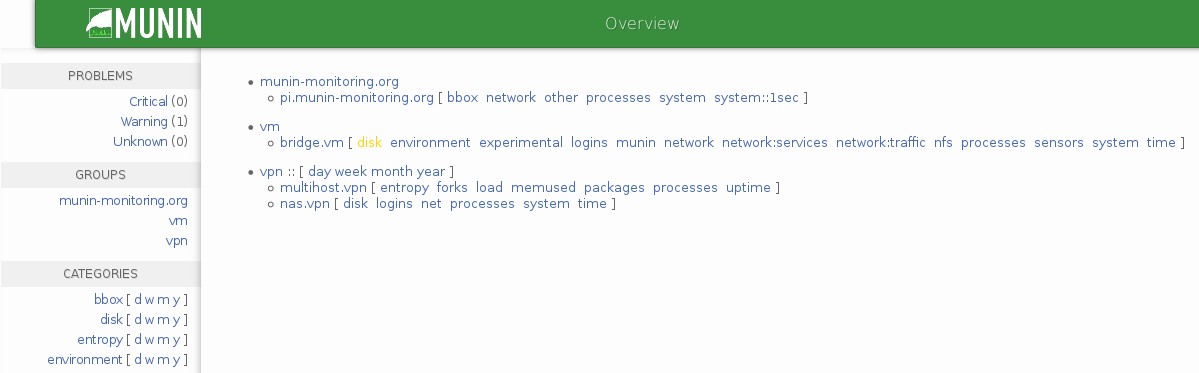
\includegraphics[width=0.7\textwidth]{20}
    \caption{Pantalla inicial de Munin}
    \label{iniciomunin}
\end{figure}

Por ejemplo, si hacemos click en la categoría \textit{processes} vemos todos los datos relacionados con procesos que ha obtenido Munin que en este caso serían tasa de \textit{fork} en procesos, número de hebras, prioridad de procesos, etc. Algunas de éstas gráficas de las que hablo se ven en la \hyperref[procesos]{Subfigura \ref*{procesos}}. Cada gráfico corresponde a un servidor distinto, en este caso el primero corresponde al servidor munin-monitoring.org y el segundo, al vm. Para saber esto debemos hacer click en el gráfico que queramos consultar, donde accederemos a una página similar donde se indicará ya el servidor correspondiente. En la \hyperref[fork]{Subfigura \ref*{fork}} vemos la tasa de fork para el servidor munin-monitoring.org, tenemos varias gráficas según queramos consultarlo por año, por día, por mes o por semana.

\begin{figure}[!h]
\centering
\mbox {
\subfigure[Algunos de los gráficos que vemos al acceder a la categoría de procesos]{
\label{procesos}
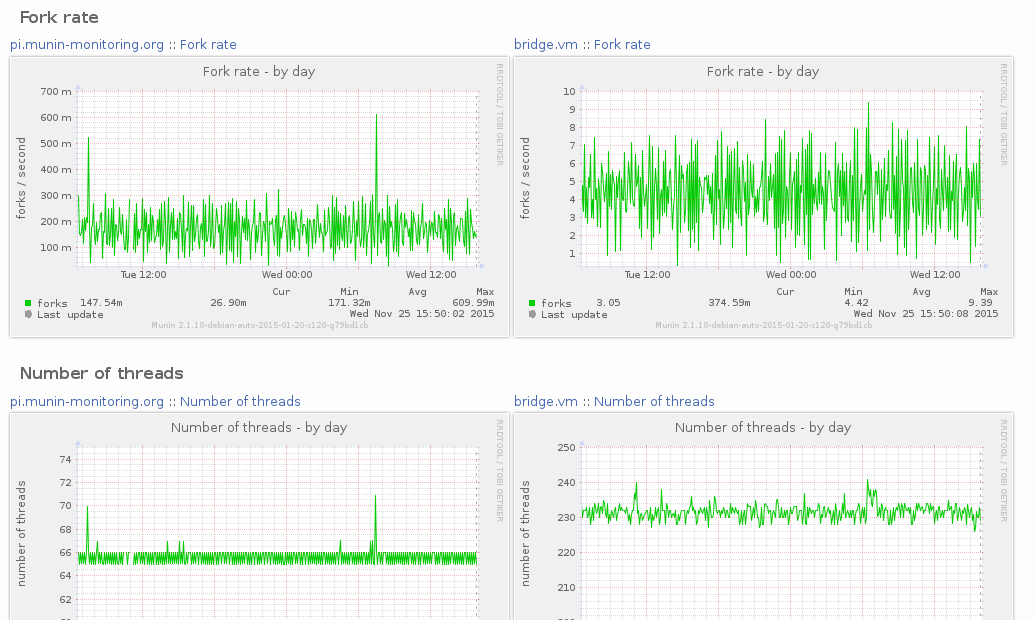
\includegraphics[width=0.5\textwidth]{21}
}
\qquad
\subfigure[Gráficos sobre la tasa de fork en el servidor munin-monitoring.org] {
\label{fork}
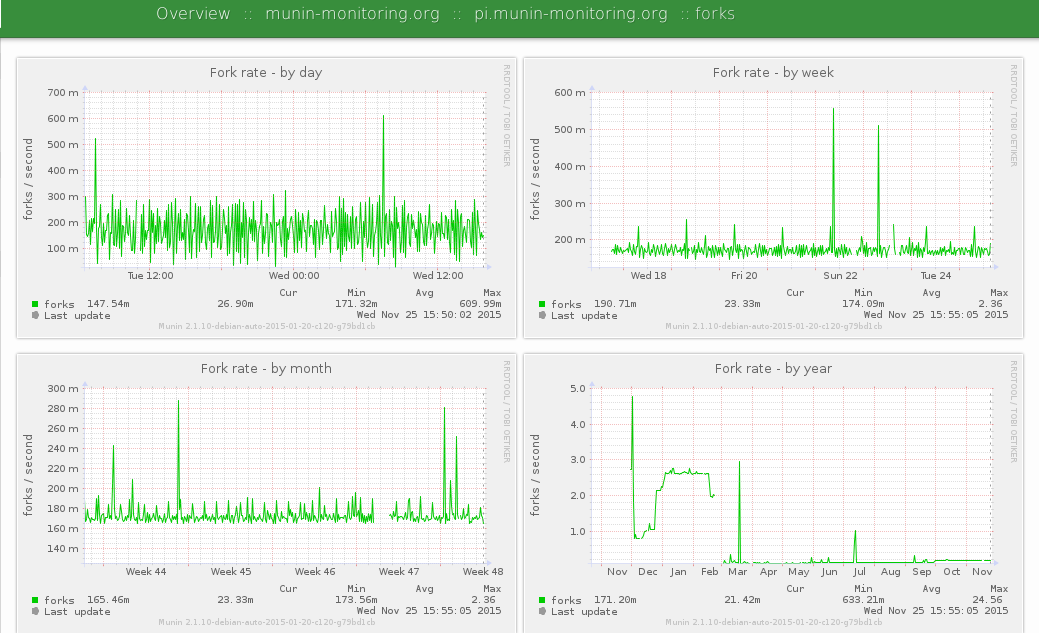
\includegraphics[width=0.5\textwidth]{22}
}
}
\caption{Consultando datos concretos en Munin}
\label{datosmunin}
\end{figure}

Si hacemos click en uno de los gráficos iremos a una página en la que podremos consultar el gráfico con detalle, ésto se ve en la \hyperref[forksdia]{Subfigura \ref*{forksdia}}. Podemos interactuar con él eligiendo con tres clicks una zona en la que queramos hacer zoom, ésto se ve en las Subfiguras \hyperref[zooming]{\ref*{zooming}} y \hyperref[zoom]{\ref*{zoom}} de la \hyperref[grafica]{Figura \ref*{grafica}}. Con el zoom podemos consultar los forks que hubo a una determinada hora (en este caso la media noche del miércoles). En este caso veríamos por ejemplo que sobre las 2:30 de la madrugada se ejecutó un proceso que tuvo muchos forks y sobre las 1:45 todo lo contrario. Observando la gráfica podemos decir que el número de forks que se hacen en el sistema es bastante cambiante.

\begin{figure}[!h]
\centering
\mbox {
\subfigure[Página detallada del gráfico de forks por día]{
\label{forksdia}
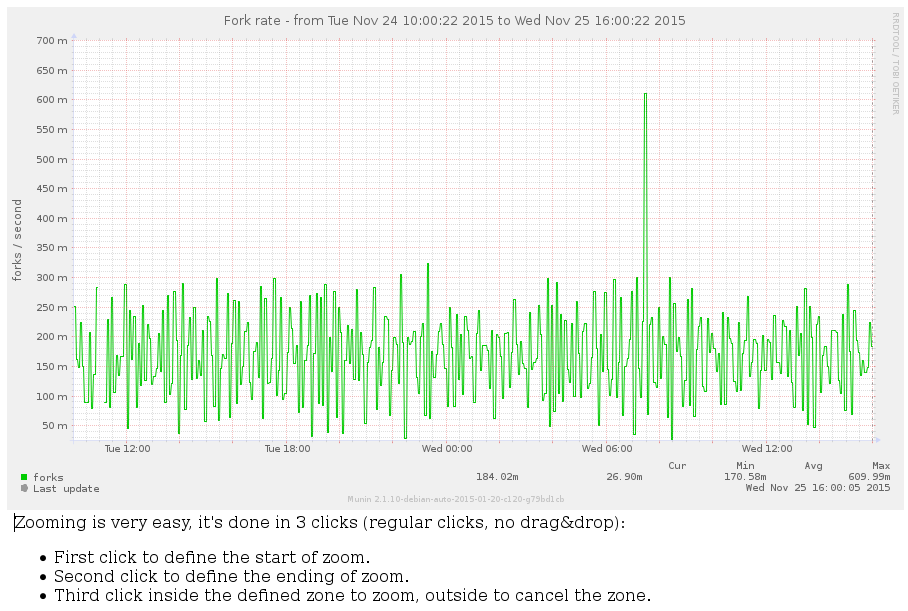
\includegraphics[width=0.5\textwidth]{23}
}
\qquad
\subfigure[Eligiendo la zona en la que queremos hacer zoom] {
\label{zooming}
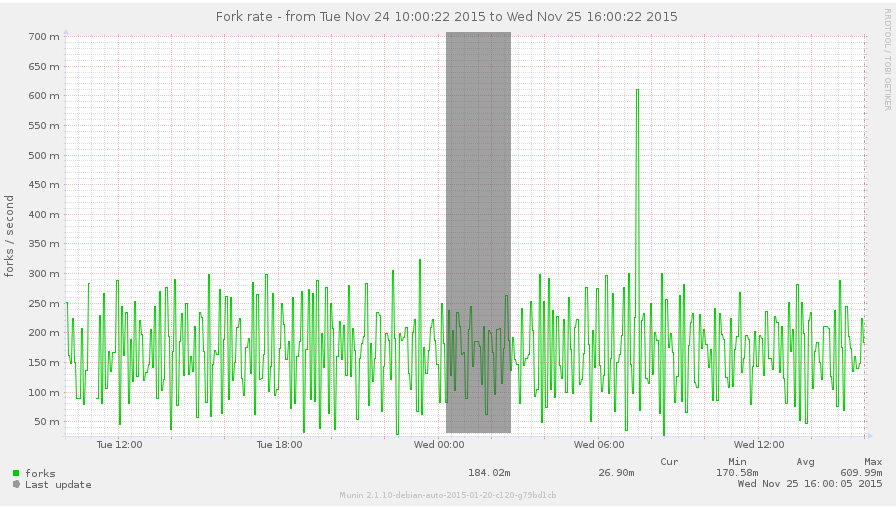
\includegraphics[width=0.5\textwidth]{24}
}
}
\subfigure[Cómo queda el gráfico tras hacer zoom en una zona] {
\label{zoom}
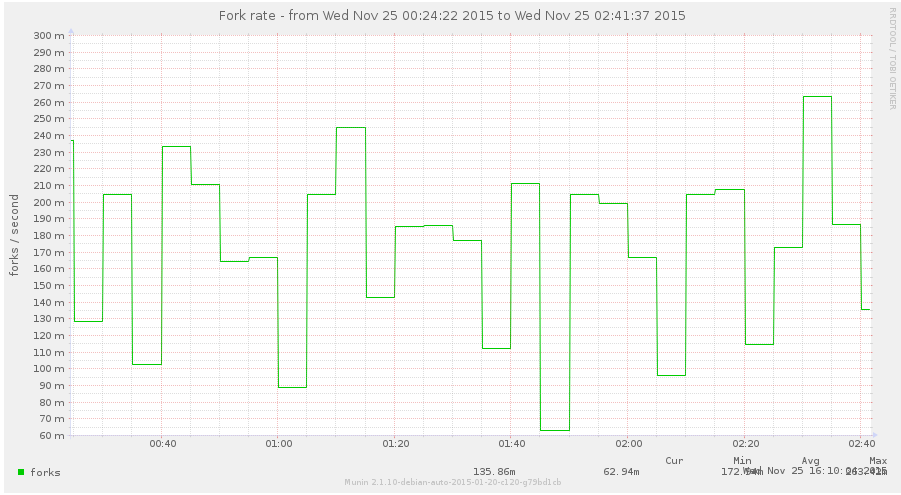
\includegraphics[width=0.5\textwidth]{25}
}
\caption{Interactuando con una gráfica}
\label{grafica}
\end{figure}

En lo que a procesos se refiere, sólo tenemos medidas del servidor vm, éstas se ven en la \hyperref[procesosvm]{Subfigura \ref*{procesosvm}}. Para monitorizar el número de procesos que ha habido en una semana hacemos click en la segunda gráfica y obtenemos la gráfica de la \hyperref[semanapr]{Subfigura \ref*{semanapr}}, en dicha gráfica vemos unos huecos que nos resultan extraños, así que hacemos zoom en uno de ellos obteniendo la gráfica de la \hyperref[raro]{Subfigura \ref*{raro}}. En ella vemos que, durante dos horas (18:00-20:00), o bien se apagó el servidor o bien se dejó de monitorizar porque no hay ningún proceso ejecutándose en el sistema. El resto del tiempo el número de procesos es bastante homogéneo, unos 200, de los cuales la mayoría son procesos suspendidos (\textit{sleeping}) y unos 5 o 6 están ejecutándose.

\begin{figure}[!h]
\centering
\mbox {
\subfigure[Gráficas obtenidas al medir el número de procesos en el servidor vm]{
\label{procesosvm}
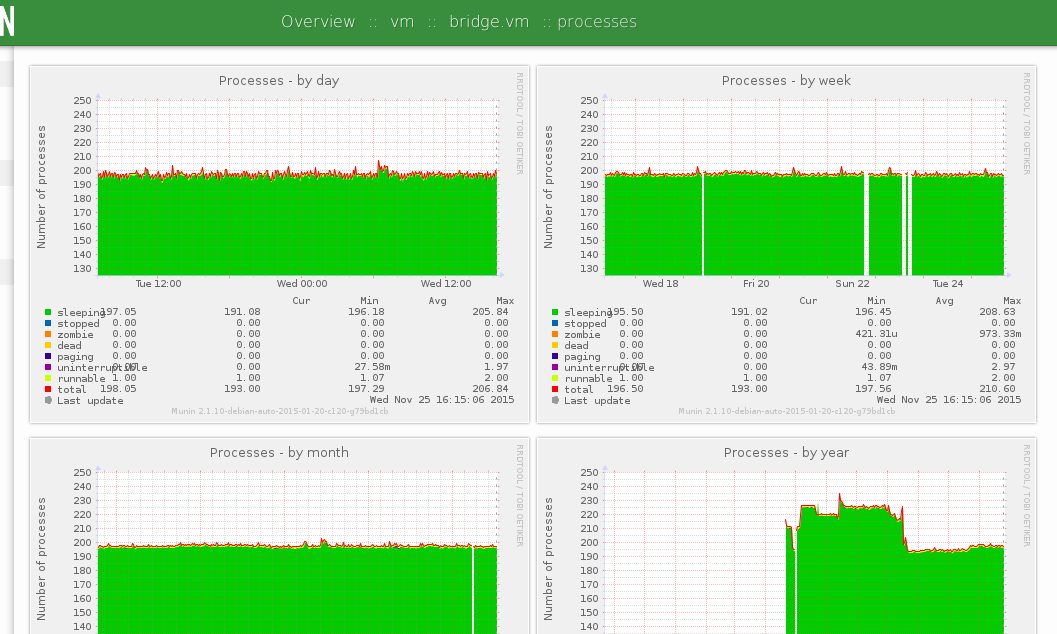
\includegraphics[width=0.5\textwidth]{26}
}
\qquad
\subfigure[Gráfica detalla sobre el número de procesos por semana] {
\label{semanapr}
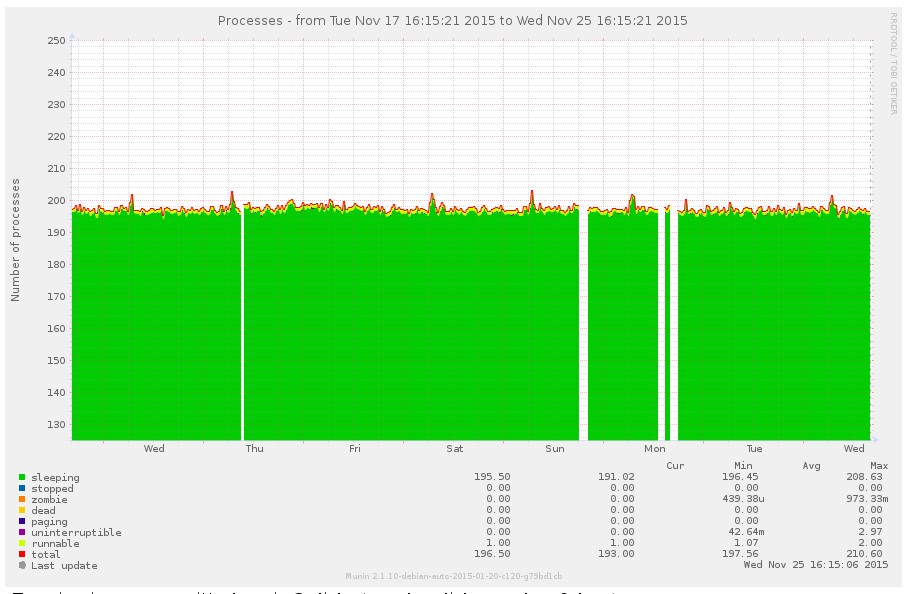
\includegraphics[width=0.5\textwidth]{27}
}
}
\subfigure[Haciendo zoom sobre una zona del gráfico que nos ha resultado algo rara] {
\label{raro}
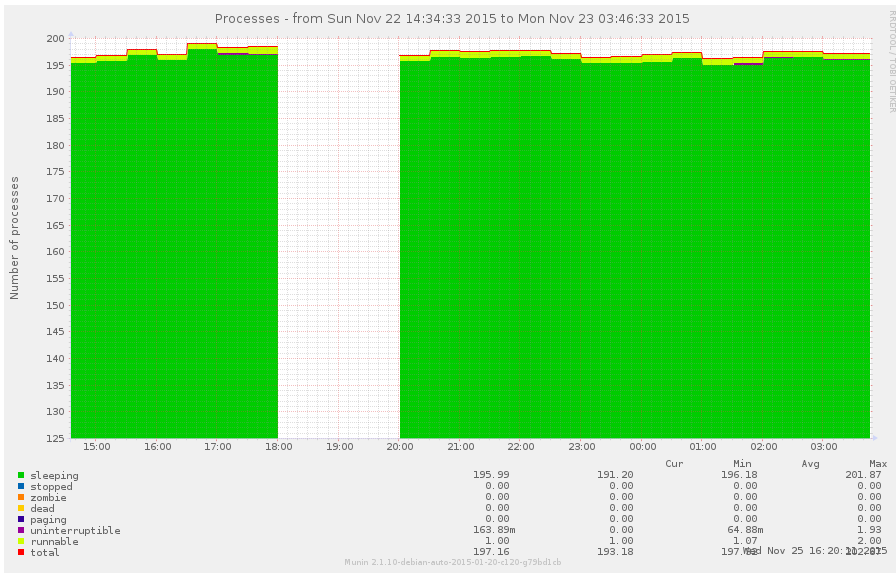
\includegraphics[width=0.5\textwidth]{28}
}
\caption{Monitorizando el número de procesos}
\label{procesosnumber}
\end{figure}

\section{Escriba un breve resumen sobre alguno de los artículos donde se muestra el uso de \texttt{strace} o busque otro y coméntelo}
El artículo consultado ha sido \cite{strace}, en él se explica la funcionalidad básica de \texttt{strace} y varios ejemplos de uso.

\texttt{strace} sirve para hacer un seguimiento de las llamadas al sistema que realiza un determinado proceso. Ésto sirve para detectar errores que no se reflejan en los archivos de logs. Sobre todo se usa para hacer seguimiento de llamadas al sistema bien conocidas tales como \texttt{open}, \texttt{close}, \texttt{read}, \texttt{write}, etc.

Para ver las llamadas al sistema realizadas al leer un archivo con \texttt{cat}, ejecutamos \texttt{strace} de la siguiente manera:
\begin{minted}[frame=single, label={Ejecutando strace}]{bash}
strace cat text.txt
\end{minted}

En la salida de dicho comando veremos, en las primeras líneas las llamadas al sistema correspondientes para ejecutar el proceso \texttt{cat}, y después, veremos las llamadas al sistema que realiza \texttt{cat} para abrir el archivo e imprimirlo por la salida estándar.

Tras explicar el ejemplo simple con \texttt{cat}, el artículo nos muestra algunos ejemplos más complejos e interesantes.

En el primero de ellos, nos muestra tres opciones de \texttt{strace}: la opción \texttt{-o}, la opción \texttt{-e} y la opción \texttt{-Ff}. La primera de ellas sirve para redirigir el output a un archivo, la segunda, para filtrar el output de tal forma que sólo veamos las llamadas al sistema \texttt{open} y la tercera, para seguir todos los procesos hijos que haga el proceso.

El segundo de ellos consiste en encontrar un fallo al iniciar un servidor Apache, dicho fallo consiste en que no puede abrir correctamente el archivo de logs, por lo que si no fuese usando \texttt{strace} no habría ninguna forma de encontrar dicho error.

Finalmente el artículo nos anima a probar \texttt{strace} mientras editamos un fichero de texto para ir viendo las llamadas al sistema ``en directo'' que vamos haciendo mientras escribimos. En la \hyperref[straceprueba]{Figura \ref*{straceprueba}} se ve mi prueba. Por cada carácter que introduzco, se hace una llamada a \texttt{read} y unas cuantas llamadas más adelante, se hace una llamada a \texttt{write}. Por último, el programa se queda esperando a que escriba otra tecla para realizar otra llamada más a \texttt{read}.

\begin{figure}[!h]
    \centering
    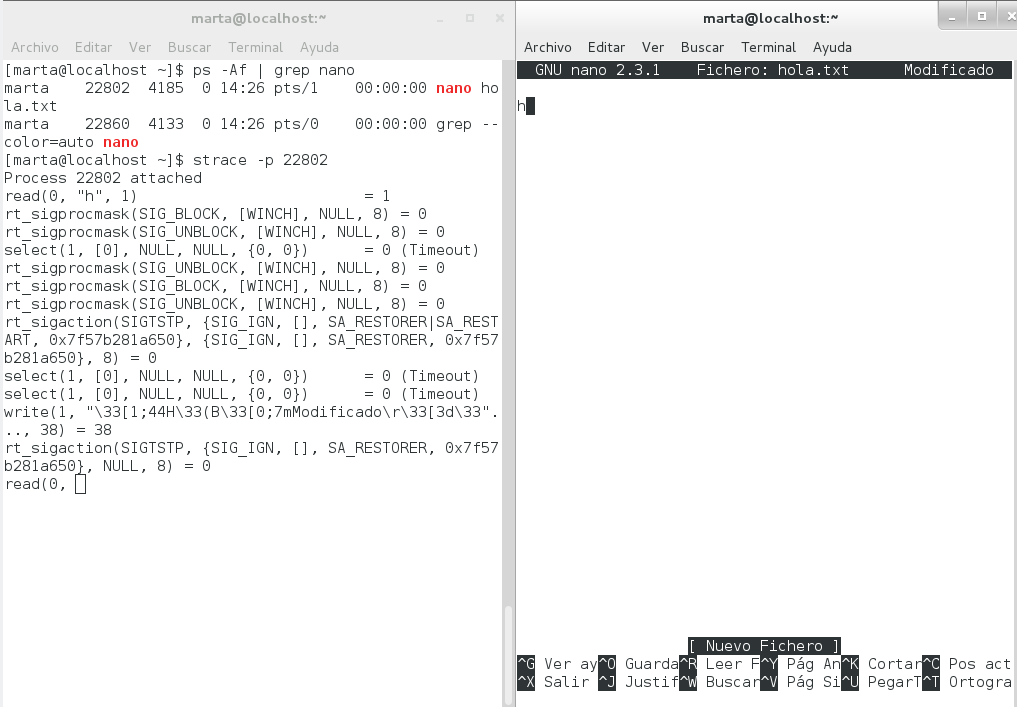
\includegraphics[width=0.7\textwidth]{39}
    \caption{Haciendo la prueba con \texttt{strace} que nos sugiere el artículo}
    \label{straceprueba}
\end{figure}

Al pulsar \textbf{Control+o} para guardar, se ha leído la tecla \texttt{"$\setminus$17"} y nos imprime por pantalla ``Nombre del fichero''. (\hyperref[guardar]{Figura \ref*{guardar}}).

\begin{figure}[!h]
    \centering
    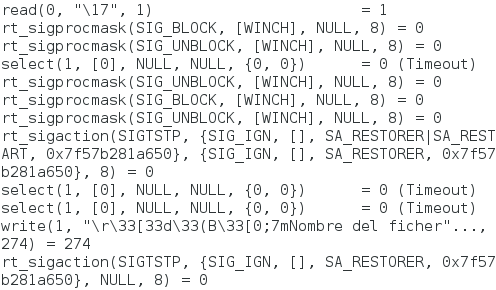
\includegraphics[width=0.5\textwidth]{40}
    \caption{Llamadas al sistema realizadas cuando vamos a guardar un fichero}
    \label{guardar}
\end{figure}

Al presionar \textbf{Enter} para guardar el fichero, intenta abrir el fichero, al no poder encontrarlo lo crea con la llamada al sistema \texttt{open}. Tras ésto escribe en el fichero el texto que hemos introducido en él con \texttt{write} y por último, lo cierra con \texttt{close} (\hyperref[fichero]{Figura \ref*{fichero}}).

\begin{figure}[!h]
    \centering
    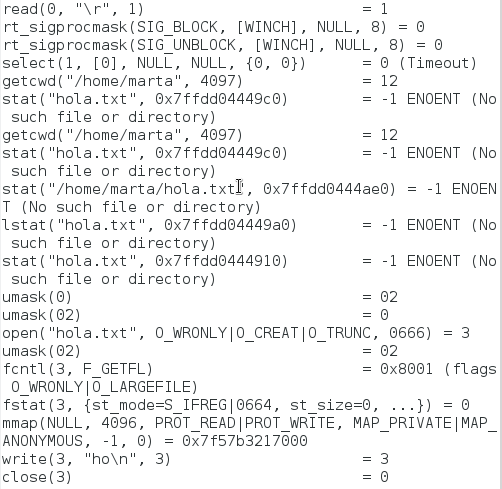
\includegraphics[width=0.5\textwidth]{41}
    \caption{Llamadas al sistema realizadas cuando guardamos un fichero}
    \label{fichero}
\end{figure}

\section{Acceda a la consola \texttt{mysql} (o a través de \texttt{phpMyAdmin}) y muestre el resultado de mostrar el ``profile'' de una consulta (la creación de la BD y la consulta la puede hacer líbremente)}
Para activar el \textit{profiling} debemos activar el \textit{flag} \texttt{profiling} (ya que por defecto su valor es 0). Ésto se hace con el siguiente comando:
\begin{minted}[frame=single, label={Activando el profiling en SQL}]{mysql}
mysql> SET profiling = 1;
\end{minted}

Así, habilitamos el profiling de cada consulta que hagamos y que luego podremos consultar con el comando \texttt{SHOW PROFILES}.

La base de datos usada es la misma que se usó para importar en la sesión anterior (\cite{testdb}). Para poder instalarla usamos el siguiente comando:
\begin{minted}[frame=single, label={Instalando la base de datos test\_db}]{bash}
mysql -h localhost -u root -p < employees.sql
\end{minted}

La parte de la izquierda nos sirve para conectarnos a nuestra base de datos (\cite{logmysql}) y la de la derecha, para instalar la base de datos de empleados.

Una vez hecho eso, entramos en la consola de MySQL, habilitamos el \textit{profiling} e indicamos a SQL que usaremos la base de datos recién instalada. Para ello, según \cite{selectdb}, usamos el siguiente comando:
\begin{minted}[frame=single, label={Indicando a SQL que use la base de datos employees}]{mysql}
mysql> USE employees;
\end{minted}

En caso de no saber cómo se llama la base de datos recién instalada, podemos usar el siguiente comando (\cite{showdb}):
\begin{minted}[frame=single, label={Consultando las bases de datos que tenemos}]{mysql}
mysql> SHOW DATABASES;
\end{minted}

La consulta usada, en base a los datos de empleados y su estructura, se basará en los empleados cuyo nombre sea \textit{Perry}. Así, obtenemos una consulta rápida (hacer una consulta sin ningún filtro tardaría demasiado tiempo):
\begin{minted}[frame=single, label={Haciendo una consulta a la base de datos}]{mysql}
mysql> SELECT * FROM employees WHERE first_name="Perry";
\end{minted}

Tras todo esto, ejecutamos el profiling y obtenemos la salida que se ve en la \hyperref[profilesql]{Figura \ref*{profilesql}}:
\begin{minted}[frame=single, label={Ejecutando el profiler de MySQL}]{mysql}
mysql> SHOW PROFILES;
\end{minted}

\begin{figure}[!h]
    \centering
    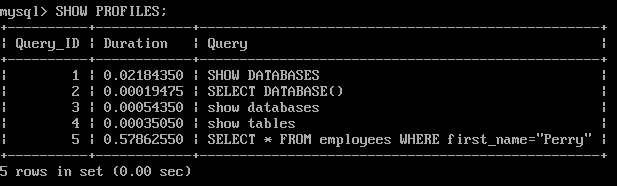
\includegraphics[width=0.7\textwidth]{43}
    \caption{Consultando los \textit{profiles} de los últimos comandos ejecutados en MySQL}
    \label{profilesql}
\end{figure}

Si comparamos cada tiempo que nos proporciona el \textit{profiler} con el tiempo que MySQL nos ha indicado vemos que ambos coinciden, aunque el tiempo indicado por el \textit{profiler} es más exacto. Por ejemplo, al finalizar la consulta a la base de datos de empleados, MySQL nos indicaba un tiempo de 0.58 segundos. Sin embargo, dicho número es redondeado, pues en realidad han sido 0.57862550 segundos.

\section{Cuestiones Opcionales}
\subsection{Indique qué comandos ha utilizado para realizar la sustitución del disco RAID1 dañado por uno nuevo así como capturas de pantalla del proceso de reconstrucción del RAID.}
Para hacerlo vamos a seguir los pasos indicados en el guión de prácticas:
\begin{enumerate}[1.]
    \item En primer lugar, vamos a la configuración de la máquina virtual y añadimos un segundo disco. Nos tiene que quedar como se ve en la \hyperref[newdisk]{Figura \ref*{newdisk}}.

    \begin{figure}[!h]
    \centering
    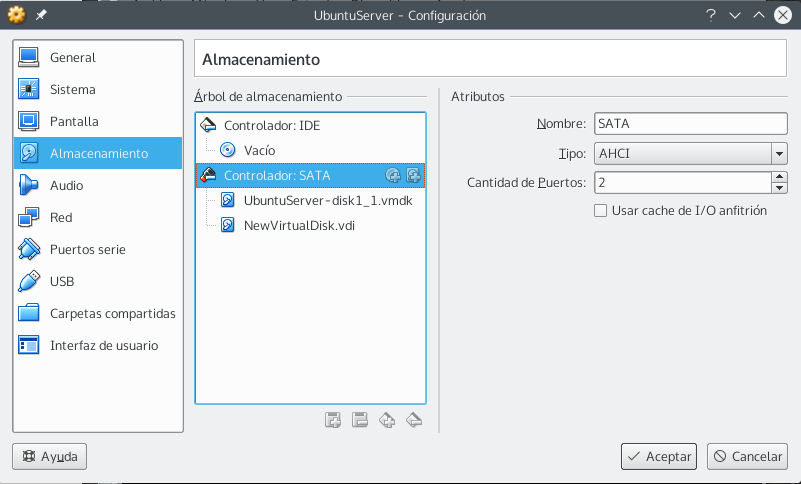
\includegraphics[width=0.7\textwidth]{3}
    \caption{Configuración de la máquina virtual tras añadir un nuevo disco}
    \label{newdisk}
    \end{figure}

    Tras añadir el disco, veremos el mensaje que se ve en la \hyperref[mensaje]{Figura \ref*{mensaje}}.
    \begin{figure}[!h]
        \centering
        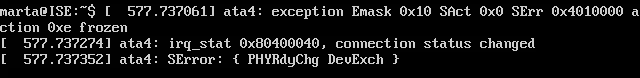
\includegraphics[width=0.7\textwidth]{4}
        \caption{Mensaje tras añadir un nuevo disco duro en caliente}
        \label{mensaje}
    \end{figure}

    \item Usamos el comando \texttt{mdadm} para eliminar el disco defectuoso del RAID y añadir el nuevo. Consultando \cite{mdadm}, vemos que para eliminar dispositivos del RAID podemos usar la opción \texttt{--remove} y para añadir, la opción \texttt{--add}.

    Primero, tenemos que consultar los discos que tenemos en nuestro ordenador, para ello usamos el comando \texttt{lsblk}. Obtenemos el output de la \hyperref[lsblk]{Figura \ref*{lsblk}}, en el cual vemos que el disco actual es el \texttt{sda1} y el que hemos insertado nuevo, \texttt{sdb}. También hemos consultado todos los dispositivos que tenemos en el sistema para saber cuál eliminar, en este caso sería \texttt{sda}.

    \begin{figure}[!h]
        \centering
        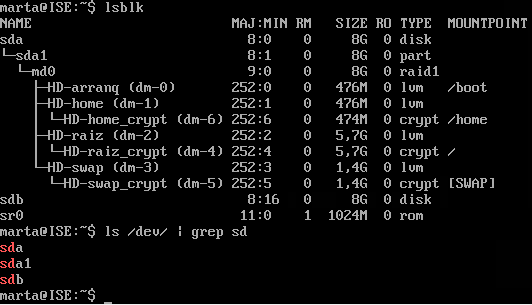
\includegraphics[width=0.7\textwidth]{5}
        \caption{Consultando cómo está el disco particionado y los discos que tenemos.}
        \label{lsblk}
    \end{figure}

    Con esa información, ejecutamos el comando \texttt{mdadm}:

\begin{minted}[frame=single, label={Eliminando el disco defectuoso y añadiendo el nuevo}]{bash}
sudo mdadm /dev/md0 --add /dev/sdb --remove /dev/sda    
\end{minted}

    Tras ejecutarlo, nos dice que se ha añadido con éxito el disco que hemos añadido nuevo, pero que no se ha encontrado el disco que íbamos a eliminar. Aún así, vemos que la ejecución ha sido exitosa en la \hyperref[finaloutput]{Figura \ref*{finaloutput}}.

    \begin{figure}[!h]
        \centering
        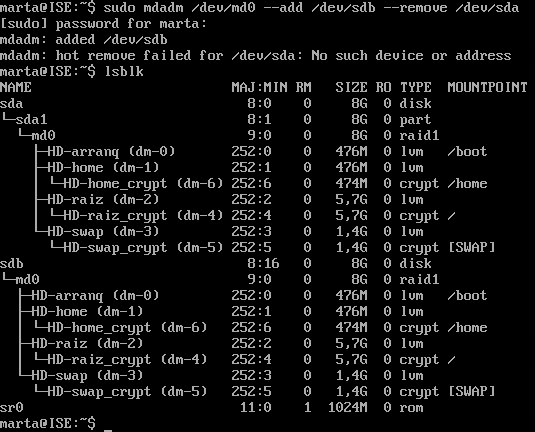
\includegraphics[width=0.7\textwidth]{6}
        \caption{Consultando cómo ha quedado particionado el disco tras añadir el disco nuevo al RAID}
        \label{finaloutput}
    \end{figure}
\end{enumerate}

\subsection{Instale \textit{Nagios} en su sistema (el que prefiera) documentando el proceso y muestre el resultado de la monitorización de su sistema comentando qué aparece.}
\subsubsection{Instalación}
En \cite{installnagios} se documenta paso a paso cómo instalar \textit{Nagios} en CentOS. Los pasos a seguir son los siguientes:
\begin{enumerate}[1.]
    \item En primer lugar, nos vamos al directorio temporal para trabajar desde ahí:
    \begin{minted}[frame=single, label={Accediendo al directorio /tmp}]{bash}
    cd /tmp
    \end{minted}

    \item Descargamos la última versión estable de \textit{Nagios}:
    \begin{minted}[frame=single, label={Descargando la última versión estable de Nagios}]{bash}
    wget http://assets.nagios.com/downloads/nagiosxi/xi-latest.tar.gz
    \end{minted}

    \item Extraemos el archivo que hemos descargado:
    \begin{minted}[frame=single, label={Extrayendo el contenido del archivo descargado}]{bash}
    tar xzf xi-latest.tar.gz
    \end{minted}

    \item Una vez extraído el archivo vamos al directorio de nagios:
    \begin{minted}[frame=single, label={Accediendo al directorio de nagios}]{bash}
    cd nagiosxi/
    \end{minted}

    \item Tras esto ejecutamos el script de instalación:
    \begin{minted}[frame=single, label={Ejecutando el script de instalación}]{bash}
    sudo ./fullinstall
    \end{minted}

    A mitad de instalación nos pedirá la contraseña para MySQL.

    \item Una vez instalado, para acceder a nagios basta con acceder a la dirección \texttt{localhost} o a la IP de nuestro servidor:
    \begin{minted}[frame=single, label={Accediendo a nagios desde Firefox}]{bash}
    firefox http://10.0.2.10/
    \end{minted}

    Una vez hecho eso, veremos la página de la \hyperref[paginicialnagios]{Figura \ref*{paginicialnagios}}.

    \begin{figure}[!h]
        \centering
        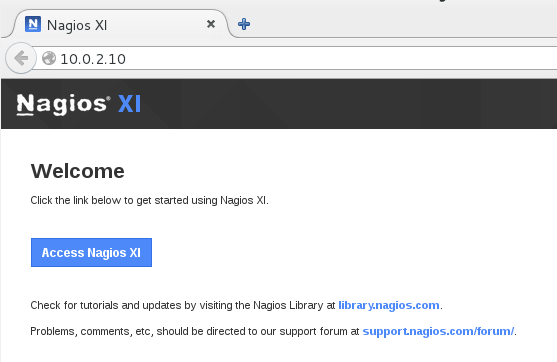
\includegraphics[width=0.5\textwidth]{29}
        \caption{Página inicial de Nagios}
        \label{paginicialnagios}
    \end{figure}

    \item Hacemos click en \textit{Access Nagios} y nos saldrá una ventana como la de la \hyperref[ventanainstall]{Figura \ref*{ventanainstall}} en la que debemos establecer algunos parámetros del sistema antes de empezar a usarlo.

    \begin{figure}[!h]
        \centering
        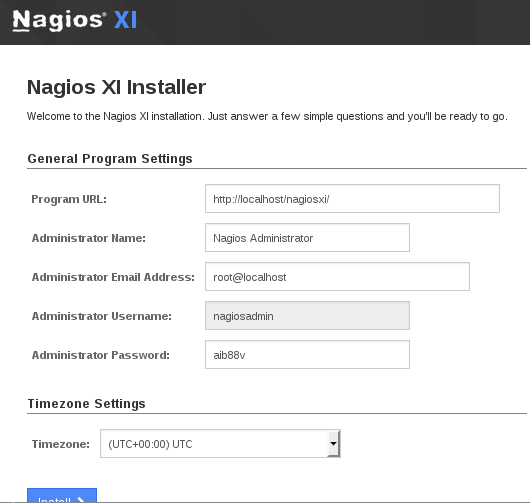
\includegraphics[width=0.5\textwidth]{30}
        \caption{Modificando algunos parámetros de Nagios antes de iniciar el sistema por primera vez}
        \label{ventanainstall}
    \end{figure}

    \item Por último nos mostrará una ventana con nuestro nombre de usuario y contraseña para acceder al sistema. Haciendo click en \textit{Login Nagios XI} e introduciendo el nombre de usuario y contraseña proporcionados, ya habremos terminado la instalación.

    \item Tras acceder al sistema deberemos de aceptar la licencia y tras aceptar la licencia nos dará un pequeño tutorial inicial. La interfaz inicial de \textit{Nagios} se ve en la \hyperref[interfaznagios]{Figura \ref*{interfaznagios}}.

    \begin{figure}[!h]
        \centering
        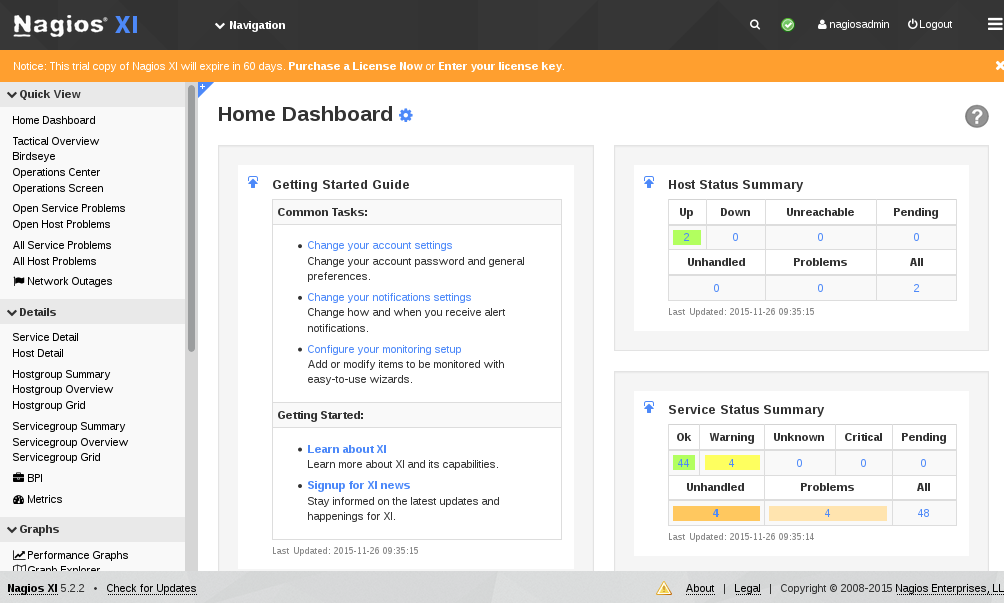
\includegraphics[width=0.5\textwidth]{31}
        \caption{Interfaz de Nagios al acceder al sistema}
        \label{interfaznagios}
    \end{figure}
\end{enumerate}

\subsubsection{Monitorización del sistema}
En el menú de la izquierda, tenemos algunas de las operaciones que podemos realizar con \textit{Nagios}. Por ejemplo, en el submení \textit{Service Detail}, podemos comprobar el estado de cada uno de los servicios que tenemos a activos en el sistema, incluyendo el propio \textit{Nagios} y el estado del propio sistema. En la \hyperref[monit]{Figura \ref*{monit}} se ve el ejemplo realizado por nosotros, en el que obtenemos varias advertencias sobre el poco espacio en disco que nos queda.

\begin{figure}[!h]
\centering
\mbox {
\subfigure[Resumen del estado de los servicios del sistema]{
\label{resumenservicios}
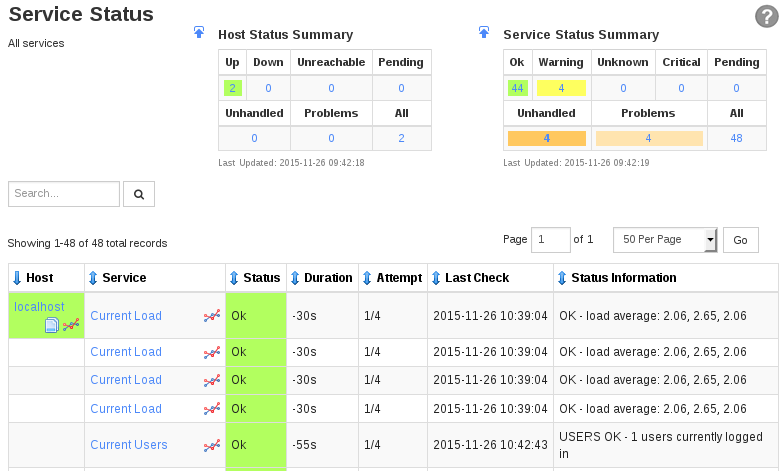
\includegraphics[width=0.5\textwidth]{33}
}
\qquad
\subfigure[Parte de la tabla detallada sobre cada servicio con varias advertencias] {
\label{advertenciasdisco}
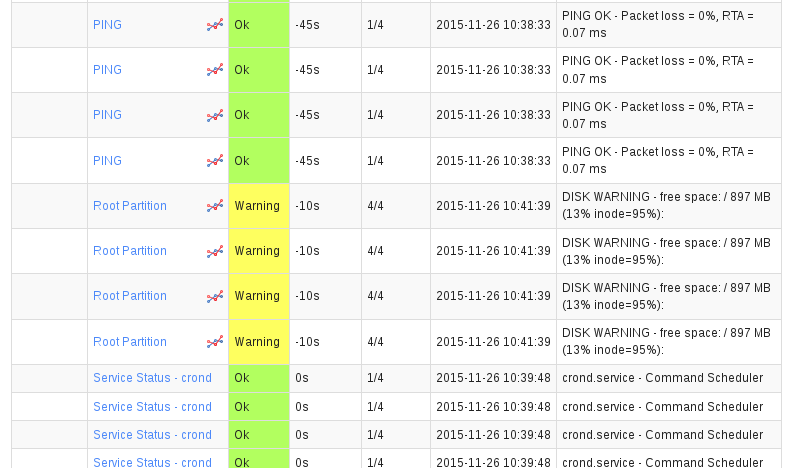
\includegraphics[width=0.5\textwidth]{32}
}
}
\caption{Monitorizando el estado de los servicios del sistema y del propio sistema}
\label{monit}
\end{figure}

En el submenú \textit{Metrics}, podemos obtener gráficas y datos sobre el uso de CPU, de memoria, de disco, de swap y la carga del sistema. En la \hyperref[swapuse]{Figura \ref*{swapuse}} estamos monitorizando el uso de la memoria de intercambio en el sistema, que en este caso vemos que tiene un uso aceptable y que no está saturada ya que tenemos un 54\% de memoria libre.

\begin{figure}[!h]
\centering
\mbox {
\subfigure[Resumen del uso de swap en el sistema]{
\label{swap}
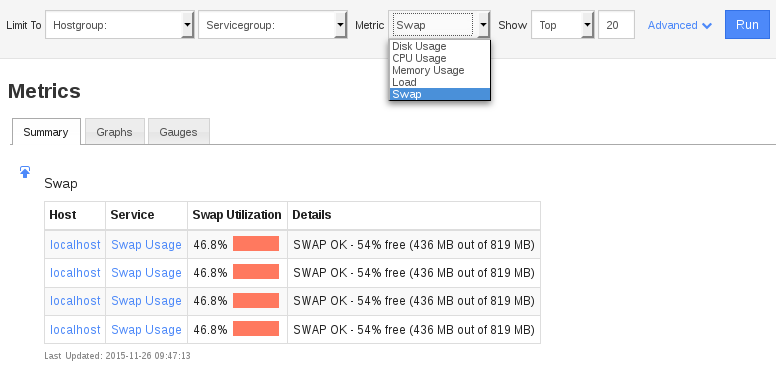
\includegraphics[width=0.5\textwidth]{34}
}
\qquad
\subfigure[Gráfica del uso de swap en el sistema] {
\label{semanapr}
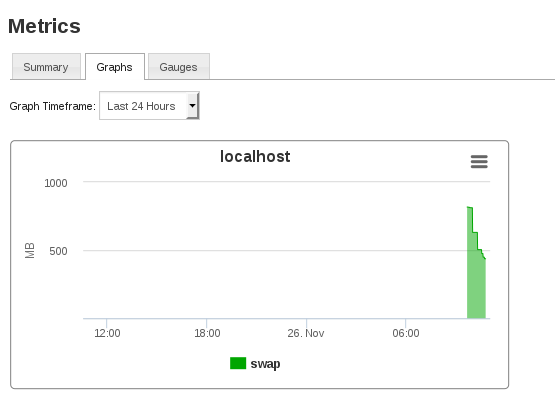
\includegraphics[width=0.5\textwidth]{35}
}
}
\caption{Monitorizando el uso de swap en el sistema}
\label{swapuse}
\end{figure}

\begin{figure}[!h]
\centering
\mbox {
\subfigure[Gráfico resumen de las veces que nuestro sistema no ha sido accesible]{
\label{salud}
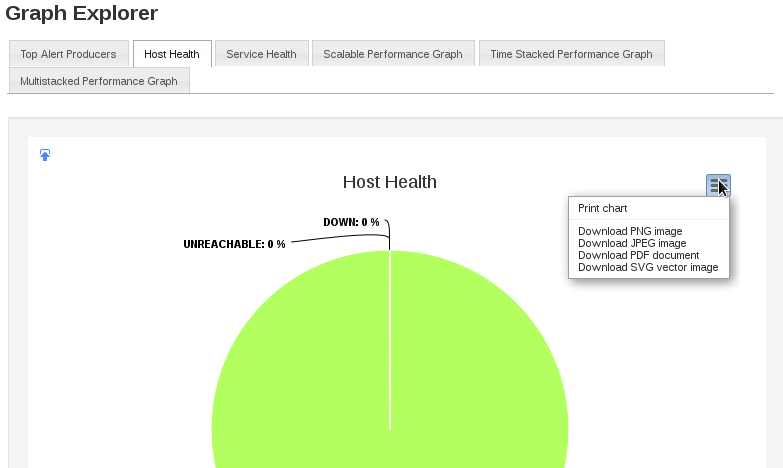
\includegraphics[width=0.5\textwidth]{37}
}
\qquad
\subfigure[Gráfico que hemos descargado en formato PNG sobre la ``salud'' de nuestro sistema] {
\label{graficopng}
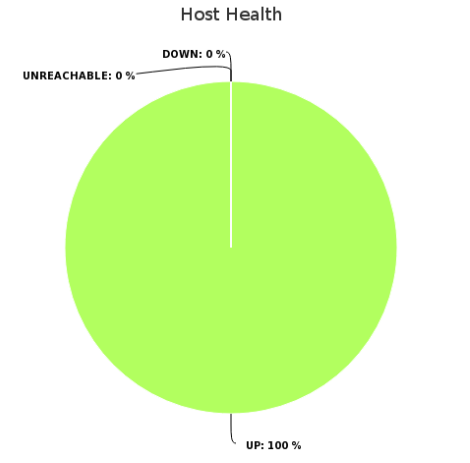
\includegraphics[width=0.3\textwidth]{38}
}
}
\caption{Monitorizando la ``salud'' del sistema}
\label{health}
\end{figure}

En el submenú \textit{Graph Explorer}, podemos consultar algunos gráficos realizados por \textit{Nagios} sobre nuestro servidor y nuestro sistema. En la \hyperref[salud]{Figura \ref*{salud}} se muestra un gráfico que muestra el número de veces que nuestro servidor ha estado innacesible (o bien porque se ha saturado, o porque se ha perdido la conexión, etc). En este caso, nuestro servidor ha estado siempre accesible y por eso muestra toda la gráfica en color verde. Además, \textit{Nagios} nos permite descargar el gráfico en varios formatos, por ejemplo en la \hyperref[graficopng]{Figura \ref*{graficopng}} se ve el archivo PNG de la gráfica descargado directamente desde \textit{Nagios}.

\subsection{Acceda a la demo online de \textit{Ganglia} de WikiMedia y haga lo mismo que hizo con \textit{Munin}}
En \href{http://ganglia.wikimedia.org/latest/}{WikiMedia} nos ofrecen una demo online del profiler \textit{Ganglia}, mostrándonos datos reales de sus servidores.

Nada más entrar a la página, nos encontramos con la página que se ve en la \hyperref[wikimediainfo]{Figura \ref*{wikimediainfo}} vemos un resumen estadístico del grid que usa WikiMedia, con el número total de CPUs y servidores tanto activos como no activos. También nos ofrecen una estadística sobre la carga desde los últimos 15 minutos y la utilización media. A la derecha de éstos datos vemos cuatro gráficas con datos sobre la carga del sistema, el uso de memoria, de CPU y de red. El uso de memoria sí es algo alto (más de la mitad), pero tanto la carga del sistema como el uso de CPU es bastante bajo. El uso de red tiene picos que varían bastante, por ejemplo, desde las 20:40 hasta las 21:00 no ha tenido actividad ninguna, sin embargo, sí ha tenido un pico de actividad a las 9.

\begin{figure}[!h]
    \centering
    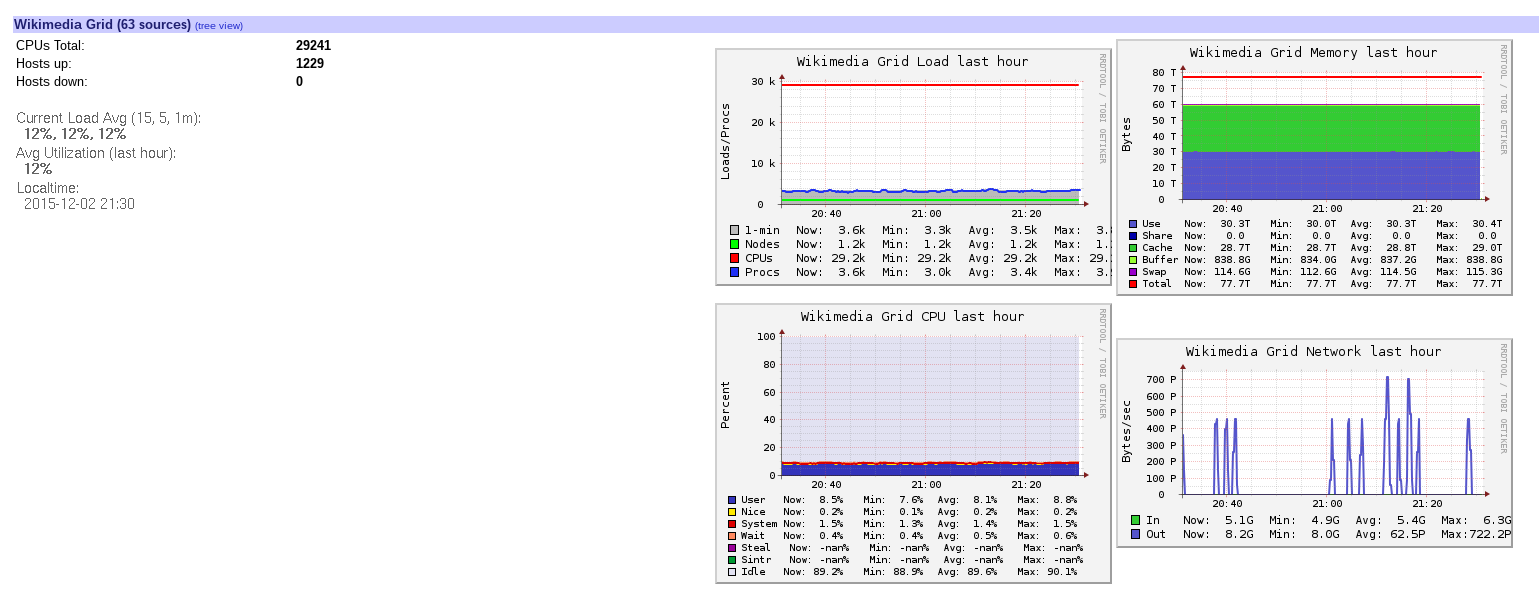
\includegraphics[width=1\textwidth]{50}
    \caption{Información general del grid de WikiMedia}
    \label{wikimediainfo}
\end{figure}

Después de esto, nos encontramos información sobre cada cluster de computadores de los que dispone WikiMedia (\textit{codfw} y \textit{equiad}). Si hacemos click en una de las gráficas, accedemos a una página en la que nos muestra información general sobre ese clúster, pero, dentro de dicha página podemos elegir ver información individual sobre un nodo concreto del clúster. Ésto se ve en la \hyperref[codfw]{Figura \ref*{codfw}}. Si elegimos un \textit{host}, vemos que tiene unas gráficas de rendimiento bastate parecidas a las del cluster (\hyperref[codfwhost]{Figura \ref*{codfwhost}}).

\begin{figure}[!h]
    \centering
    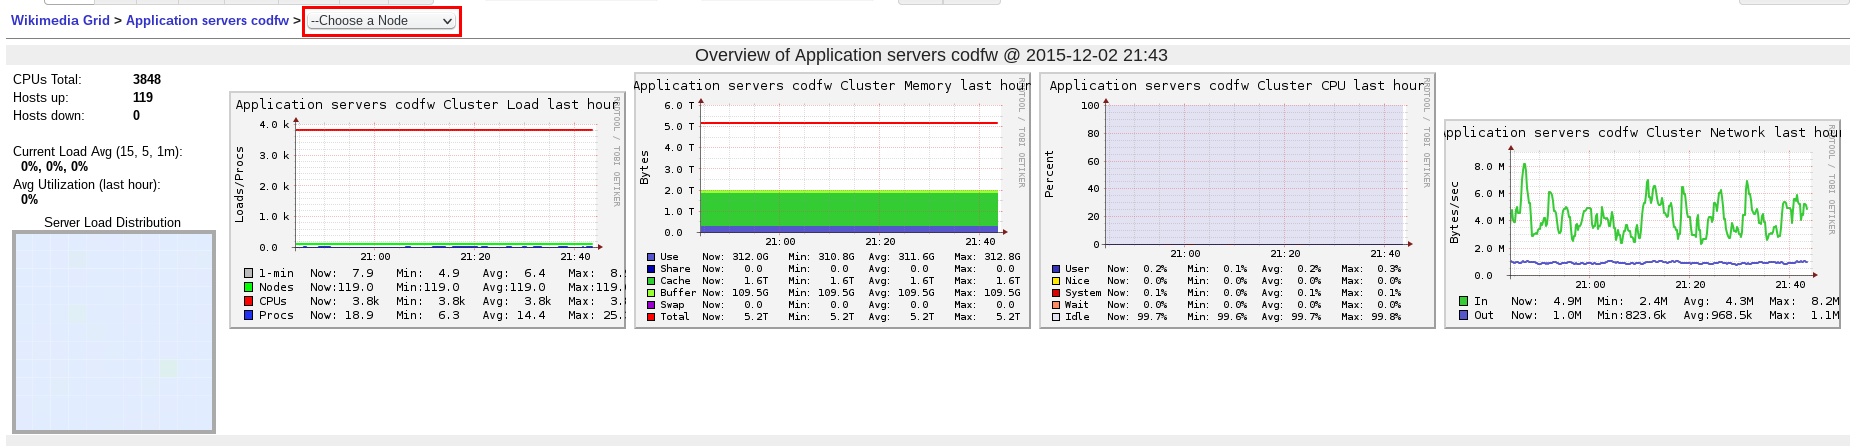
\includegraphics[width=1\textwidth]{51}
    \caption{Información general sobre los servidores de aplicación del clúster codfw}
    \label{codfw}
\end{figure}

\begin{figure}[!h]
    \centering
    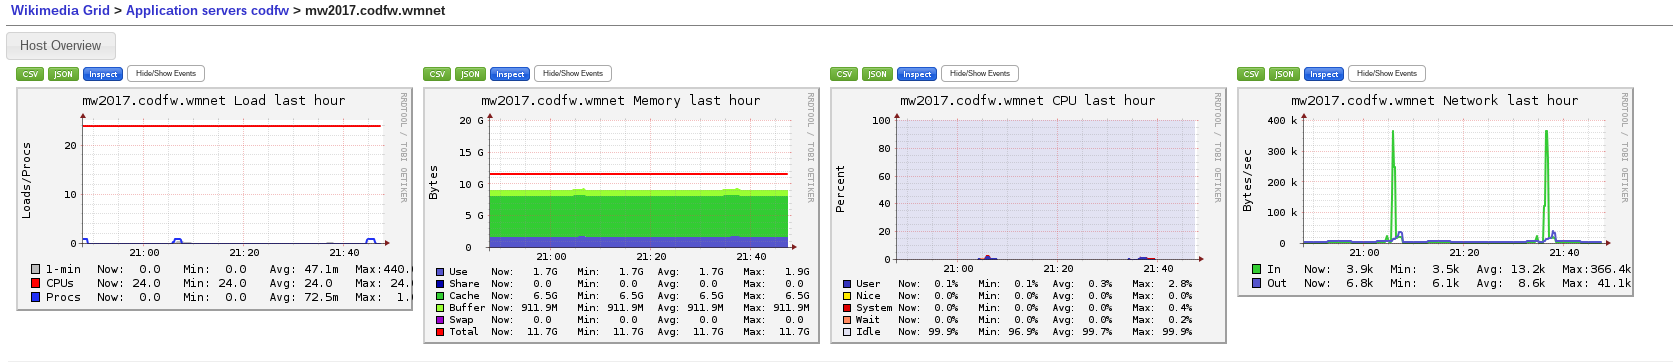
\includegraphics[width=1\textwidth]{52}
    \caption{Información general sobre uno de los hosts del clúster codfw}
    \label{codfwhost}
\end{figure}

\setcounter{subsection}{8}
\subsection{Escriba un script en python y analice su comportamiento usando el profiler presentado}
El script realizado consiste en cifrar usando el código de Polibio\cite{polibio}. El script en cuestión es el siguiente:

\mypython[label={polibio.py}]{polibio.py}

Para hacer el profiling he usado la librería \textit{cProfile}, la cual, según \cite{pyprofile}, se usa con el siguiente comando:

\begin{minted}[frame=single,label={Haciendo profile a un script en Python}]{bash}
python -m cProfile polibio.py
\end{minted}

de forma análoga también podemos usar la librería \textit{profile}, con la cual obtenemos también la misma salida.

Tras ejecutar el comando anterior, he obtenido la salida que se ve en la \hyperref[outputprofile]{Figura \ref*{outputprofile}}. En primer lugar, el \textit{profiler} nos muestra el número de llamadas a funciones que ha realizado nuestro programa y el tiempo total de ejecución. El tiempo es tan alto debido a que también cuenta el tiempo que el programa ha estado dormido esperando la entrada desde teclado.

Por último, nos muestra cada una de las funciones a las que ha llamado nuestro programa junto al número de veces que se ha llamado a cada función. Por ejemplo, las dos funciones que incluye el script (\texttt{descrifrado\_colibio} y \texttt{cifra\_polibio}) se llaman una única vez cada una, como debe de ser pues en el script sólo se hace una llamada a cada función. También se reflejan llamadas a métodos primitivos de Python tales como \texttt{index}, \texttt{append}, etc los cuales se llaman más veces debido a que se llaman dentro de bucles \texttt{for}, en concreto, números relacionados con el tamaño de la frase a cifrar introducida.

\begin{figure}[!h]
    \centering
    \includegraphics[width=1\textwidth]{42}
    \caption{Salida obtenida tras ejecutar \textit{cProfile} sobre un script Python}
    \label{outputprofile}
\end{figure}

\bibliography{P3-MarGomMac.bib} %archivo citas.bib que contiene las entradas 
\bibliographystyle{siam} % haycle varias formas de citar

\end{document}